\chapter{Definição, histórico e paradigmas}
\label{cap:introducao}

\framebox[\textwidth]{
	\hspace{1em}
	\vbox{
		\textbf{Leitura obrigatória:}
		\begin{itemize}
			\item \cite{RusselAndNorvig2010} -- Cap. 1 (Introdução).
			\item \cite{RusselAndNorvig2010} -- Cap. 26 (Fundamentos filosóficos).
		\end{itemize}
		
		\textbf{Leitura complementar:}
		\begin{itemize}
			\item \cite{RusselAndNorvig2010} -- Cap. 27 (IA, presente e futuro).
		\end{itemize}
	}
}

\section{Conceitos fundamentais}

A inteligência artificial (IA) busca \textbf{compreender} e \textbf{construir} entidades inteligentes. A questão que surge é: o que é inteligência? Ou ainda, o que faz um ser humano ser considerado um ser inteligente?
	
Na busca de uma definição mais detalhada, a IA pode ser conceituada sob duas dimensões:
\begin{itemize}
	\item \textbf{Pensamento} (como a entidade processa as informações).
	\item \textbf{Comportamento} (como a entidade atua).
\end{itemize}

Neste sentido, uma entidade pode pensar como um ser humano, ou agir como um ser humano. Estas seriam condições suficientes para classificarmos a entidade como inteligente. Porém, um ser humano é passível de erro, como tomar uma decisão ruim ou resolver um cálculo de forma incorreta. Além disso, o ser humano pode deixar-se levar por emoções e sensações na execução de uma atividade. Em alguns casos, deseja-se que uma entidade seja o mais correta possível, tomando a melhor decisão ou resolvendo corretamente um problema, por exemplo. Neste caso, deseja-se que a entidade pense racionalmente, ou aja racionalmente.

Logo, uma entidade é dita inteligente se ela pensa/age como um humano, ou se ela pensa/age racionalmente. As definições de IA são comumente formuladas conforme estas dimensões.

\insertspace

\begin{center}
	\begin{tabular}{l|l|l}
		\hline
		\textbf{SISTEMAS QUE...} & \textbf{COMO SERES HUMANOS} & \textbf{RACIONALMENTE} \\
		\hline
		\textbf{PENSAM} & \cite{Bellman1978} & \cite{Winston1992} \\
		\hline
		\textbf{ATUAM} & \cite{KurzweilEtAl1990} & \cite{PooleEtAl1998} \\
		\hline
	\end{tabular}
\end{center}

\insertspace

\begin{itemize}
	\item \textbf{\cite{Bellman1978}:} ``[Automatização de] atividades que associamos ao pensamento humano, atividades como a tomada de decisões, a resolução de problemas, o aprendizado ...''
	
	\item \textbf{\cite{KurzweilEtAl1990}:} ``A arte de criar máquinas que executam funções que exigem inteligência quando executadas por pessoas.''
	
	\item \textbf{\cite{Winston1992}:} ``O estudo das computações que tornam possível perceber, raciocinar e agir.''
	
	\item \textbf{\cite{PooleEtAl1998}:} ``A Inteligência Computacional é o estudo do projeto de agentes inteligentes.''
\end{itemize}

\insertspace

\section{Teste de Turing}

O Teste de Turing foi proposto por Alan Turing (1950) com o objetivo de fornecer uma definição operacional de inteligência. Ou seja, melhor do que definir um conjunto de características para classificar uma entidade como inteligente ou não, ele propôs um teste que, quando aprovado, indica que a entidade é inteligente.

\textbf{Ideia geral:} um ser humano interroga, através de um teclado, duas entidades ocultas: um ser humano e um computador. O computador passa no teste quando, após algumas perguntas, o interrogador não puder identificar qual das duas entidades é o humano (veja ilustração da Figura~\ref{fig:teste-turing}).

\begin{figure}[H]
	\centering
	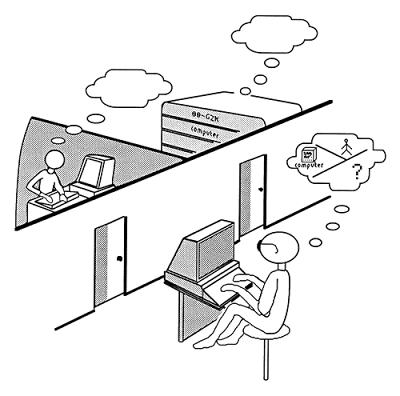
\includegraphics[width=0.6\textwidth]{img/teste-turing}
	\caption{Ideia geral do Teste de Turing}
	\label{fig:teste-turing}
\end{figure}

Logo, o Teste de Turing avalia se uma entidade é inteligente de acordo com a dimensão ``\textit{a entidade se comporta como um humano}''. O teste não avalia se a máquina pensa como um ser humano, pois não tem acesso à forma como a resposta foi inferida. Também não avalia a racionalidade, uma vez que:
\begin{itemize}
	\item O interrogado (seja o computador ou o humano) pode errar a resposta de alguma pergunta.
	\item Pode tomar uma decisão errada, ou não optar pela melhor decisão possível.
\end{itemize}

\insertspace

Até o momento, nenhuma máquina passou no teste, que ganhou popularidade por exigir uma série de capacidades da IA:
\begin{itemize}
	\item Processamento de linguagem natural
	\item Representação do conhecimento
	\item Raciocínio automatizado
	\item Aprendizagem de máquina
\end{itemize}
	
\insertspace
	
Considere as perguntas a seguir. Elas são simples de responder, mas não tão triviais a um computador.
\begin{itemize}
	\item Por que os cachorros não voam no inverno?
	\item O que você acha da papelaria de Presidente Getúlio?
\end{itemize}

\section{Hipóteses da IA}

Uma abordagem mais filosófica da IA sugere duas hipóteses: IA fraca e IA forte. A hipótese da IA fraca sugere que as máquinas podem \textbf{agir de maneira inteligente} (ou agir como se fossem inteligentes). A hipótese da IA forte sugere que as máquinas agem de forma inteligente porque \textbf{podem pensar} (quando o fazem, estão realmente pensando como um ser humano ou um ser racional).

\textbf{Em resumo:} simulação de inteligência (IA fraca) \textit{versus} inteligência real (IA forte).

\subsection{IA Fraca}
A IA fraca simula o pensamento ou comportamento inteligentes. Isto é, esta hipótese não se importa se a máquina está de fato pensando, ou se apenas segue um modelo que a leva para o resultado desejado. Esta hipótese preocupa-se em apresentar um comportamento inteligente. O Teste de Turing se preocupa em identificar entidades que são dotadas de inteligência seguindo esta abordagem. A pregunta que esta vertente busca responder é: \textit{as máquinas podem agir com inteligência}?

\subsection{IA Forte}

A IA forte visa o desenvolvimento de máquinas auto-conscientes. Ou seja, máquinas que efetivamente podem pensar. Esta abordagem considera ainda que a entidade, no seu processo cognitivo, é capaz de sentir, contêm emoções e são capazes de expressá-las. A pergunta que esta vertente busca responder é: \textit{as máquinas podem realmente pensar}? Como esperado, esta abordagem gera muitas discussões em torno da real possibilidade de se concretizar no futuro. Além disso, outros questionamentos se baseiam na ética em torno dos seus objetivos.

\section{Histórico}

A partir de 1943 alguns pesquisadores se dedicavam a estudar conceitos que se tornariam as bases para o que conhecemos hoje por inteligência artificial. Este período é chamado de \textit{gestação} da IA, que nasce no ano de 1956. A partir disso, foram anos de desenvolvimento acelerado da área e resultados otimistas. Mesmo assim, a área sofreu um período difícil pela dificuldade em tratar problemas reais, gerando perda de investimentos. Finalmente, a IA torna-se comercial principalmente pelos sistemas de apoio à tomada de decisão, bem como torna-se uma área de pesquisa científica, resultando no cenário atual. Abaixo apresenta-se um resumo da evolução da IA e dos seus principais marcos ao longo dos anos.

\insertspace

\begin{itemize}
	\item \textbf{1943:} modelagem de um neurônio artificial por Warren McCulloch e Walter Pitts e a ideia de simular o funcionamento do cérebro com uma rede de neurônios.
	
	\item \textbf{1950:} apresentação de uma visão completa da IA por Alan Turing, no seu artigo ``Computing Machinery and Intelligency''. Foram apresentados os conceitos de aprendizagem de máquina, algoritmos genéticos e aprendizagem por reforço.

	\item \textbf{1951:} primeira rede neural (SNARC), por Mrvin Minsky e Dean Edmonds.
	
	\item \textbf{1952:} aplicação de IA em jogos (damas, por exemplo), utilizando conceitos de aprendizagem de máquina, por Arthur Samuel.
	
	\item \textbf{1956:} considerado o nascimento da IA, por conta de um seminário organizado em Dartmouth College.
	\begin{itemize}
		\item Destaque para o programa de raciocínio \textit{Logic Theorist} (LT), criado por Allen Newell e Herbert Simon.
	\end{itemize}
	
	\item \textbf{1958:} John McCarthy cria a linguagem Lisp e, com ela, cria o primeiro sistema de IA completo: Advice Taker.
	\begin{itemize}
		\item Conceitos de representação do conhecimento e raciocínio.
	\end{itemize}
	
	\item \textbf{1960's:} rápida evolução das técnicas através da aplicação em problemas específicos, chamados \textit{minimundos}.
	\begin{itemize}
		\item Paralelo a isso, os pesquisadores perceberam que os métodos desenvolvidos eram limitados e resolver problemas da prática era um desafio ainda distante de ser alcançado.
		\item Exemplos: problemas com explosão combinatória; tradução de documentos.
	\end{itemize}
	
	\item \textbf{1970's:} incorporação de conhecimento do domínio para a resolução de problemas.
	\begin{itemize}
		\item Conceito de sistemas especialistas, que utilizam a representação do conhecimento e estratégias de raciocínio que exploram este conhecimento.
		\item Aplicações: DENDRAL, MYCIN.
	\end{itemize}
	
	\item \textbf{1980:} IA como uma indústria (aplicações comerciais).
	\begin{itemize}
		\item R1: primeiro sistema especialista comercial (1982).
		\item Grandes corporações investiam em um setor de IA, economizando milhões de dólares por ano.
	\end{itemize}
	
	\item \textbf{1987:} IA como uma ciência.
	\begin{itemize}
		\item Base nos fundamentos e teorias de outras áreas correlatas.
		\item Evolução dos métodos e bons resultados.
	\end{itemize}
	
	\item \textbf{1995:} conceito de agentes inteligentes.
	\begin{itemize}
		\item Formalização de uma estrutura para sistemas inteligentes.
		\item Um agente se divide em percepção, raciocínio e ação.
	\end{itemize}
	
	\item \textbf{1997:} Deep Blue versus Kasparov em uma disputa de xadrez.
	\begin{itemize}
		\item Kasparov: ``Senti uma nova espécia de inteligência do outro lado do tabuleiro.''
	\end{itemize}
	
	\item \textbf{2004:} agentes inteligentes na exploração espacial.
	
	\item \textbf{2007:} veículos autônomos.
	
	\item \textbf{2017:} uma máquina (AlphaGo) vence o melhor jogador de Go do mundo.
\end{itemize}


\section{Paradigmas}

Existem três paradigmas para a inteligência artificial: simbólico, conexionista e evolutivo. Estes paradigmas direcionam as pesquisas para a construção de sistemas inteligentes e apresentam técnicas sob diferentes perspectivas. A IA acabou dividindo-se em diferentes paradigmas por pesquisadores explorá-la através de diferentes caminhos: a IA deve se basear no estudo da psicologia (forma como entidades inteligentes raciocinam) ou da biologia (funcionamento estruturas biológicas que permitem o raciocínio)?

\subsection{IA simbólica}
Se baseia na representação do conhecimento através de símbolos. Este conhecimento é manipulado e, sobre ele, são realizadas inferências para a geração de novos conhecimentos. O exemplo mais comum de método simbólico na IA são os sistemas especialistas. As principais técnicas utilizadas são a lógica (proposicional e de primeira ordem) e a otimização.

\subsection{IA conexionista}
Se baseia na construção de sistemas inteligentes com base no funcionamento do cérebro humano, seus neurônios e conexões neurais. A inteligência do sistema emerge do funcionamento individual de cada neurônio, bem como da comunicação entre eles. Logo, este ramo é representado pelas redes neurais.

\subsection{IA evolutiva}
Este paradigma sugere que um sistema pode evoluir, de tal forma a tornar-se mais inteligente. Ou ainda, seus métodos propõem a evolução de soluções para problemas específicos. Esta evolução é obtida através de recombinações e mutações. O ramo mais conhecido deste paradigma são os algoritmos genéticos (bem como programação genética).

\section{Recursos disponíveis}

Existem softwares para uso pessoal que adotam técnicas de inteligência artificial no seu funcionamento interno. Exemplos são os assistentes pessoais que qualquer pessoa pode ter em seu smartphone ou computador. A Apple possui a Siri~\footnote{\url{https://support.apple.com/pt-br/HT204389}}, enquanto a Microsoft possui o Cortana~\footnote{\url{https://www.microsoft.com/pt-br/windows/cortana}} e a Google possui o Google Now~\footnote{\url{https://www.google.com/intl/pt-BR/landing/now/}}. Aplicações com inteligência artificial das mais diversas naturezas também estão disponíveis a usuários finais. Esta postagem~\footnote{\url{https://goo.gl/zXTnE8}} apresenta algumas delas.

Por outro lado, também existem diversas ferramentas para suporte a desenvolvedores que desejam construir aplicações com recursos de inteligência artificial. O PredictionIO~\footnote{\url{http://predictionio.incubator.apache.org}} é um servidor de aprendizagem de máquina para a criação de motores de predição. O Eclipse Deeplearning4j~\footnote{\url{https://projects.eclipse.org/proposals/eclipse-deeplearning4j}} é uma biblioteca de \textit{deep learning} para desenvolvedores Java com uma série de recursos disponíveis. A Microsoft apresenda o Azure~\footnote{\url{https://azure.microsoft.com/pt-br/overview/ai-platform/}}, que dentre uma série de outros recursos, possui uma plataforma de inteligência artificial com diversos serviços para desenvolvedores. Protégé~\footnote{\url{https://protege.stanford.edu}} é um framework para desenvolvimento de sistemas inteligentes baseados em conhecimento e que utilizem ontologias para sua representação. O Watson~\footnote{\url{https://www.ibm.com/watson/}} da IBM é uma plataforma que disponibiliza uma variedade de ferramentas de inteligência artificial, com exemplos de código e aplicações tanto para desenvolvedores como usuários finais. O DiffBlue~\footnote{\url{http://www.diffblue.com/}} é uma ferramenta para automação de código, que oferece serviços como localização de erros, refatoração de código e testes. O TensorFlow~\footnote{\url{https://www.tensorflow.org/}} da Google é uma plataforma para projetos de aprendizagem de máquina que disponibiliza uma variedade de recursos para desenvolvedores. O Nervana Neon~\footnote{\url{https://ai.intel.com/neon/}} é uma bilbioteca em Python para aprendizagem de máquina. Finalmente, o Neural Designer~\footnote{\url{https://www.neuraldesigner.com/}} é uma ferramenta que fornece suporte a tarefas de aprendizagem de máquina baseadas em redes neurais.

Ao longo dos capítulos seguintes, serão apresentados recursos específicos para os conteúdos estudados neste material, os quais poderão ser utilizados no desenvolvimento e solução dos exercícios propostos.

\section{Exercícios}

\begin{exercise}
Defina com suas próprias palavras: (a) inteligência, (b) inteligência artificial e (c) racionalidade.
\end{exercise}

\begin{exercise}
Suponha que a inteligência artificial seja utilizada para desenvolvimento de um sistema que atinja um grau 200 em um teste padrão de QI. Nesse caso, teríamos um programa mais inteligente que um ser humano? Explique.
\end{exercise}

\begin{exercise}
Até que ponto os sistemas seguintes são instâncias de inteligência artificial?
\begin{itemize}
	\item Leitores de código de barra de supermercados.
	\item Menus de voz de telefones.
	\item Mecanismos de busca na Web.
	\item Algoritmos de roteamento da Internet que respondem dinamicamente ao estado da rede.
\end{itemize}
\end{exercise}

\begin{exercise}
Todo ano o prêmio Loebner é entregue ao programa que chega mais perto de ser aprovado em uma versão do teste de Turing. Pesquise sobre o último vencedor do prêmio Loebner, comentando sobre os conceitos de inteligência artificial utilizados por ele.
\end{exercise}

\begin{exercise}
Examine a literatura de IA para descobrir se as tarefas a seguir podem ser resolvidas atualmente por computadores. Após isso, comente sobre as dificuldades das tarefas inviáveis.

\begin{enumerate}[a.]
	\item Jogar uma partida de tênis de mesa.
	\item Dirigir no centro do Cairo, Egito.
	\item Comprar mantimentos para uma semana no mercado.
	\item Comprar mantimentos para uma semana na Web.
	\item Jogar uma partida decente de \textit{bridge} em nível competitivo.
	\item Descobrir e provar novos teoremas matemáticos.
	\item Escrever uma história intencionalmente engraçada.
	\item Dar assessoria jurídica competente em uma área especializada de direito.
	\item Traduzir o inglês falado ao sueco falado, em tempo real.
	\item Executar uma operação cirúrgica complexa.
\end{enumerate}

\end{exercise}